\documentclass{article}

\usepackage[vmargin=4cm]{geometry} % paginamarge
\usepackage{geometry} % paginamarge
\usepackage[dutch]{babel} % Nederlandse dingen
\usepackage{enumerate} % Geavanceerde lijsten
\usepackage{amssymb} % Wiskundige symbolen
\usepackage{graphicx} % Plaatjes!
\geometry{a4paper}
\usepackage{fancyhdr} % Mooie pagina's (met lijntje)
\pagestyle{fancy}

\fancyhead[LO]{}
\fancyhead[CO]{Prototype selection through proximity graphs}
\fancyhead[RO]{}

\title{Prototype selection for the nearest neighbour rule through proximity graphs}
\author{Mathijs Vos \and Ramon Janssen \and Petra van den Bos}

\begin{document}
\maketitle
\tableofcontents
\newpage

\begin{abstract}
Het k-nearest-neighbour-principe kan ge\"implementeerd worden door gebruik te maken van proximity graphs. Van de trainset wordt een graaf gemaakt waarbij de buren van een punt kunnen stemmen volgens het kNN-principe. Bij proximity graphs kan eerste orde en tweede orde editing toegepast worden, wat invloed heeft op welke punten kunnen stemmen in kNN.

	In dit verslag worden Gabriel Graphs en Relative Neighbourhood Graphs besproken, en hoe hier door middel van editing en condensing een prototype van te maken is. De implementatie hiervan is getest op een aantal testsets en de resultaten hiervan worden genoemd en besproken. Tot slot worden de voor- en nadelen van dit algoritme besproken.
\end{abstract}

\section{Inleiding}
Een belangrijk probleem in data-analyse is dat van classificatie. Hoe deel je verschillende objecten of personen in, op basis van bepaalde kenmerken? Hiervoor is in de classificatie een algemeen stappenplan beschikbaar: van een aantal gevallen worden de kenmerken bepaald, en deze worden stuk voor stuk handmatig ingedeeld in een categorie. Een programma gebruikt deze gegevens als trainset, en verwerkt deze gegevens. Het programma kan daarna van onbekende gevallen de klasse voorspellen, als de kenmerken gegeven worden. Hierbij is te denken aan het classificeren van plaatjes op basis van hun pixels, het stellen van een diagnose op basis van medische kenmerken, en vele andere soorten problemen.

Een veelgebruikt criterium om punten te classificeren is het k-nearest-neighbour-principe. Hierbij wordt het k aantal punten bekeken dat het dichts bij het te testen punt ligt. Dit kan gedaan worden met de euclidische afstand van alle eigenschappen, maar dit verschilt per implementatie. De "buren" die zo gevonden worden, stemmen over welke klasse het nieuwe punt moet zijn. Het kNN-principe kan gemakkelijk worden toegepast op verschillende soorten datasets, doordat de afstand gemakkelijk onafhankelijk van het aantal punten en het aantal eigenschappen van de punten kan worden berekend.


\section{Het Probleem}
\subsection{Condensing en editing}

Het kNN-principe kan op een simpele manier op alle soorten gegevens worden toegepast. Door een nieuw punt simpelweg met alle punten in de trainset te vergelijken kan een goed resultaat worden verkregen. In de praktijk levert dit echter problemen op in performance, omdat een dataset al snel veel dimensies en punten bevat. Ook wordt ruis daarmee overgenomen, omdat van elk punt van de trainset wordt aangenomen dat deze correct gelabeld is. De complexiteit voor het testen van nieuwe punten wordt dan al snel veel te groot en daardoor zijn optimalisaties vereist.

Het doel van condensing is om de grootte van een dataset te reduceren door redundante informatie te schrappen. Dit richt zich voornamelijk op gebieden waar zich veel punten met dezelfde klasse bevinden: de punten in het midden van het gebied voegen niets toe ten opzichte van de punten op de rand. Alleen de randen worden dus gespaard. Hierbij zorgt ruis voor een probleem, omdat \'{e}\'{e}n (verkeerd gelabeld) punt in het midden van een gebied er anders voor zou zorgen dat het midden niet meer condensed kan worden.
	
Voor het weghalen van ruis is er editing. Dit haalt punten weg die nabij veel punten met een andere classificatie liggen, omdat dit soort punten meer kans hebben om ruis te zijn. Dit kan het beste v\'{o}\'{o}r het condensen gebeuren, zodat de condensing minder last heeft van ruis.
	
Voor zowel condensing als editing kan de precieze werking verschillen. Het is afhankelijk van het algoritme hoeveel informatie er verwijderd wordt. Als er meer informatie verwijderd wordt, worden de resultaten gemiddeld slechter maar wordt de benodigde tijd voor het testen minder. Het verschilt ook per algoritme hoe effectief editing en condensing is onder verschillende omstandigheden, zoals de hoeveelheid dimensies en de vorm van de data.

\subsection{De methode}
De titel van het artikel dat wij gekozen hebben is ``Prototype selection for the nearest neighbour rulethrough proximity graphs''. We hebben dit artikel gekozen omdat het ons wel leuk leek om grafen te gebruiken en omdat het artikel duidelijk was. Er worden twee soorten grafen beschreven: \emph{Gabriel Graphs} en \emph{Relative Neighbourhood Graphs}. Beiden zijn grafen waarin punten verbonden worden door lijnen die elkaar niet snijden. Als een punt A verbonden is met punt B, is A een buur van B en B een buur van A.

\subsubsection{Gabriel Graph}
In een Gabriel Graph is er een verbinding tussen twee punten, als binnen de cirkel, waarvan de verbinding de diameter is, geen andere punten liggen. Met de euclidische afstand kan dit formeel uitgedrukt worden: A en B hebben een verbinding als voor alle andere punten X geldt: ${afstand^2}(A,B) \leq {afstand^2(A,X)} + {afstand^2}(B,X)$. In Figuur \ref{GGburen} zijn A en B verbonden, maar B en C niet. In Figuur \ref{graaf_xor_GG} is een gehele Gabriel Graph te zien. \\

\begin{figure}[!h]
    \centering
        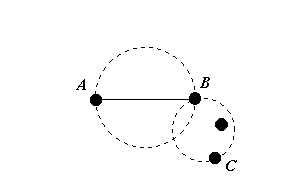
\includegraphics[scale=1, page=1]{GGburen}
    \caption{Buren van punten in een Gabriel Graph}
    \label{GGburen}
\end{figure}

\begin{figure}[!h]
    \centering
        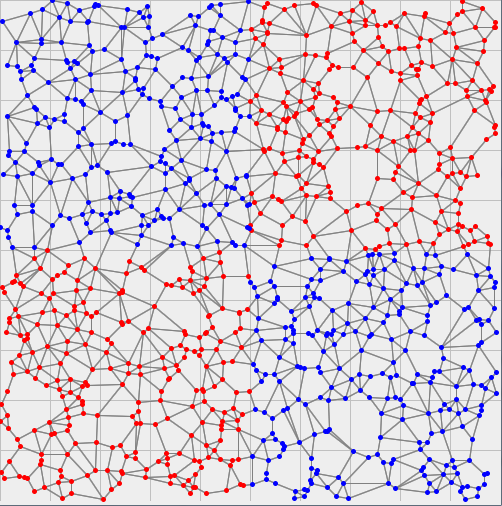
\includegraphics[scale=0.5, page=1]{graaf_xor_GG}
    \caption{Een Gabriel Graph}
    \label{graaf_xor_GG}
\end{figure}
\clearpage

\subsubsection{Relative Neighbourhood Graph}
In een Relative Neighbourhood Graph hebben twee punten een verbinding als er geen andere punten binnen de `lune' van die twee punten liggen, zie Figuur 3. Met de euclidische afstand kan dit formeel uitgedrukt worden: A en B hebben een verbinding als voor alle andere punten X geldt: $afstand(A,B) \leq max\{afstand(A,X),afstand(B,X)\}$. In Figuur \ref{RNGburen} zijn B en C  verbonden, maar A en B niet. In Figuur \ref{graaf_xor_RNG} is een gehele Relative Neighbourhood Graph te zien.\\

\begin{figure}[!h]
    \centering
        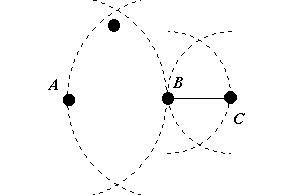
\includegraphics[scale=1, page=1]{RNGburen}
    \caption{Buren van punten in een Relative Neighbourhood Graph}
    \label{RNGburen}
\end{figure}
\begin{figure}[!h]
    \centering
        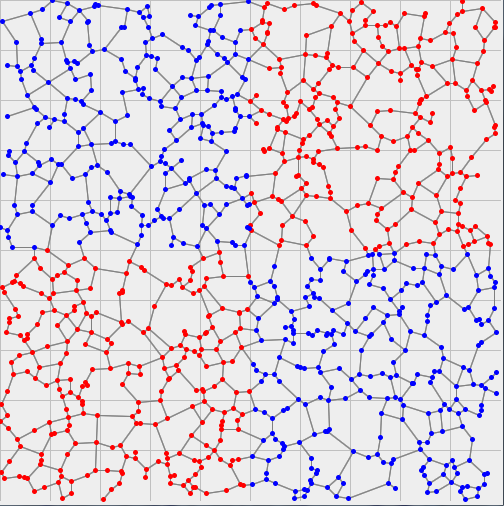
\includegraphics[scale=0.5, page=1]{graaf_xor_RNG}
    \caption{Een relative neighbourhood graph}
    \label{graaf_xor_RNG}
\end{figure}
\clearpage

Deze grafen kun je gebruiken om nieuwe data (de testset) te klassificeren aan de hand van data waarvan de classificatie al bekend is (de trainset). Een graaf bevat in eerste instantie dus alle punten uit de trainset. Om de performance te verbeteren en eventuele ruis te compenseren, wordt condensing en editing toegepast op de trainset. Hierbij wordt gekeken naar de punten die een verbinding hebben met een bepaald punt. Bij condensing wordt ieder punt weggehaald, dat alleen verbindingen naar punten met dezelfde klasse heeft. 
In het artikel werden twee soorten editing algoritmes besproken: een eerste orde editing algoritme en een tweede orde editing algoritme. 
Het eerste orde editing algoritme bepaalt voor elk punt of de meerderheid van de buren van dat punt tot een van de andere klasses behoort. De punten waarvoor dit geldt, worden verwijderd. 
Het tweede orde algoritme verwijdert alle punten als geldt dat de meerderheid van de buren tot een van de andere klasses behoort, en als ook de meerderheid van de buren, van de buren die van dezelfde klasse als dat punt zijn, tot een van de andere klasses behoort.\\

De testset wordt geklassificeerd op de volgende manier: Eerst wordt de graaf van alle punten van de trainset geconstrueerd. Vervolgens wordt eerste of tweede orde editing toegepast. Daarna wordt condensing toegepast. Met de bewerkte graaf die overblijft wordt een klasse aan elk van de punten in de testset toegewezen. Dit gebeurt met behulp van het k-nearest neighbour algoritme. Van elk punt in de testset wordt gekeken welke k punten het dichtstbij liggen. Deze k dichtstbijzijnde punten bepalen we door ofwel alleen naar de directe buren van het testsetpunt te kijken (eerste orde), ofwel naar de directe buren en buren van die directe buren te kijken (tweede orde). Als k groter is dan het aantal buren dat het testsetpunt heeft, worden alleen die buren gebruikt. Daardoor is k voor dat punt dus kleiner.

\section{Experimenten}

We hebben onze methode met verschillende datasets getest:
\begin{enumerate}
\item De XOR-dataset met 2 dimensies en 2 mogelijke klasses.
\item De MNIST-dataset met 196 dimensies en 10 mogelijke klasses.
\item De diabetes-dataset met 8 dimensies en 2 mogelijke klasses.
\end{enumerate}

\subsection{XOR}
We hebben de gemiddelde nauwkeurigheid en reductie voor elk ruispercentage bepaald, door het gemiddelde te nemen van de score van alle testsets (dat waren er 40), toegepast op alle trainsets (er waren 10 trainsets). Hierbij hebben we Gabriel Graphs gebruikt. We hebben deze tests gedaan voor eerste orde en tweede orde editing, in combinatie met eerste orde en tweede orde (k-nearest-neighbour) tests op de punten van de testset. Hieronder staan de testresultaten weergegeven in een tabel en daarbij twee grafieken die de resultaten uit de tabel weergeven.

\subsubsection{Eerste orde editing, eerste orde tests}
\begin{tabular}{|c|c|c|c|} \hline
Ruis & K=1 & K=3 & K=5 \\ \hline
0\% &	92,99 &	90,17 &	88,58 \\
10\% &	91,37 &	88,69 &	86,94 \\
20\% &	86,78 &	86,07 &	84,62 \\
30\% &	75,71 &	73,76 &	72,91 \\
40\% &	65,18 &	66,11 &	65,31 \\
Gem.	& 82,41 &	80,96 &	79,67 \\
Gem. tot 20\%  ruis &	90,38 &	88,31 &	86,71 \\ \hline
\end{tabular} \\

\begin{center} 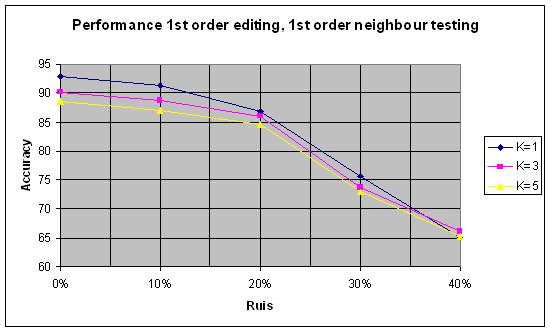
\includegraphics[scale=0.7]{xor_1stordedit_1stordtest_lijn} \end{center}
\begin{center} 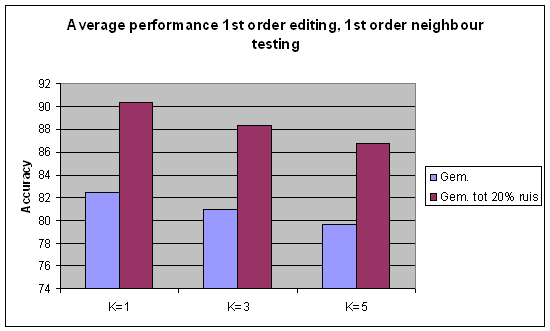
\includegraphics[scale=0.7]{xor_1stordedit_1stordtest_staaf} \end{center}

\subsubsection{Tweede orde editing, eerste orde tests}
\begin{tabular}{|c|c|c|c|} \hline
Ruis &	K=1 &	K=3 &	K=5 \\ \hline
0\% &	93,00 &	92,17 &	91,30 \\
10\%	 & 88,78 & 	89,20 &	88,21 \\
20\%	 & 82,08	& 82,72	& 82,34 \\
30\%	 & 70,84	& 71,06 &	70,4 \\
40\%	 & 61,82	 & 62,33 &	61,93 \\
Gem.	& 79,30	& 79,5 &	78,83 \\
Gem. tot 20\% ruis &	87,95 &	88,03 &	87,28 \\ \hline
\end{tabular} \\

\begin{center} 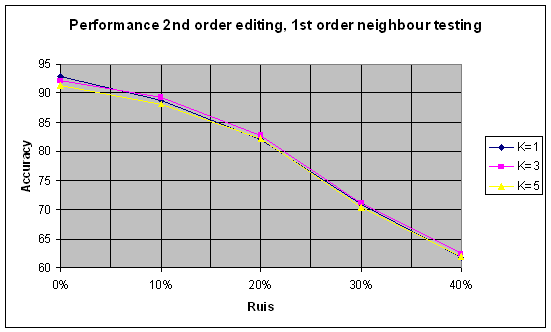
\includegraphics[scale=0.7]{xor_2ndordedit_1stordtest_lijn} \end{center}
\begin{center} 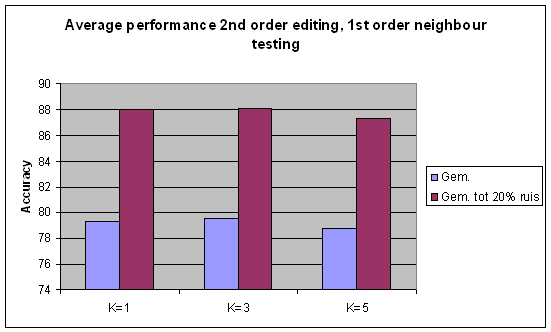
\includegraphics[scale=0.7]{xor_2ndordedit_1stordtest_staaf} \end{center}

\subsubsection{Eerste orde editing, tweede orde tests}

\begin{tabular}{|c|c|c|c|} \hline
Ruis &	K=1 &	K=3 &	K=5 \\ \hline
0\% &	92,99 &	89,94 &	86,51 \\
10\%	 & 91,37 & 	89,29 &	84,86 \\
20\%	 & 86,78 & 	84,17 &	83,49 \\
30\%	& 75,71 & 	74,83 &	75,49 \\
40\% & 65,18	& 66,72 &	69,54 \\
Gem.	& 82,41	& 80,99 &	79,98 \\
Gem. tot 20\% ruis &	90,38 &	87,80 &	84,95 \\ \hline
\end{tabular} \\

\begin{center} 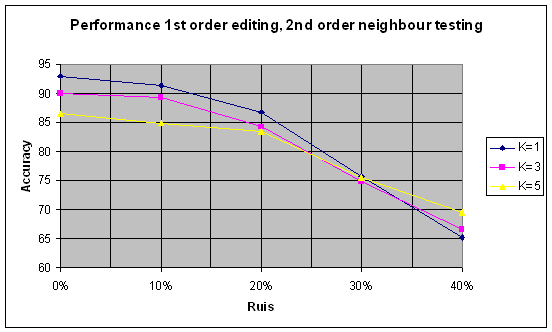
\includegraphics[scale=0.7]{xor_1stordedit_2ndordtest_lijn} \end{center}
\begin{center} 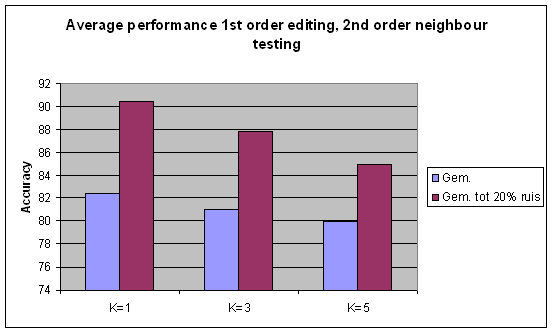
\includegraphics[scale=0.7]{xor_1stordedit_2ndordtest_staaf} \end{center}

\subsubsection{Tweede orde editing, tweede orde tests}

\begin{tabular}{|c|c|c|c|} \hline
Ruis &	K=1 &	K=3 &	K=5 \\ \hline
0\%	& 93,005 &	90,06 &	86,76 \\
10\%	 & 88,78 &	88,25 &	85,98 \\
20\%	 & 82,08 &	82,46 &	82,4 \\
30\%	 & 70,84 &	73,93 &	75,73 \\
40\%	 & 61,82 &	62,23 &	64,6 \\
Gem.	 & 79,30 &	79,38 &	79,09 \\
Gem. tot 20\% ruis &	87,95 &	86,92 &	85,04 \\ \hline
\end{tabular} \\

\begin{center} 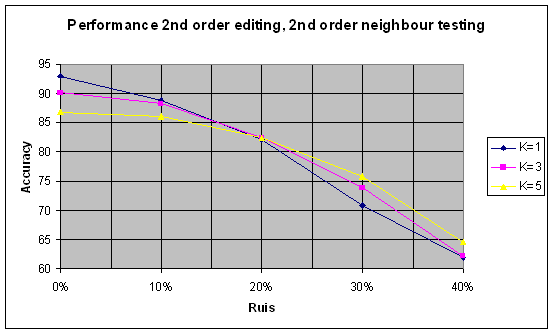
\includegraphics[scale=0.7]{xor_2ndordedit_2ndordtest_lijn} \end{center}
\begin{center} 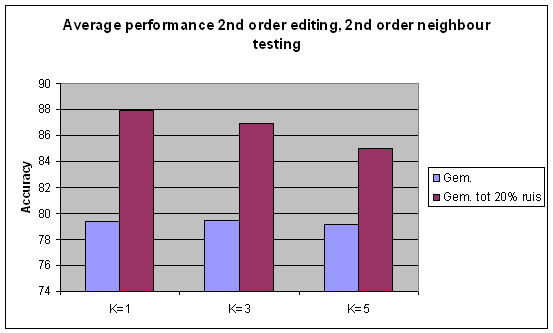
\includegraphics[scale=0.7]{xor_2ndordedit_2ndordtest_staaf} \end{center}

\subsubsection{Reductie}
\begin{tabular}{|c|c|c|c|c|c|}  \hline
&	0\% &	10\% & 	20\%	 & 30\%	 & 40\% \\ \hline
2nd order editing &	69,7 &	59,3 &	54,6 & 	56 &	50 \\
1st order editing &	75,6 &	73,1 &	74,9 &	75,9 &	70,9 \\ \hline
\end{tabular} \\
\begin{center} 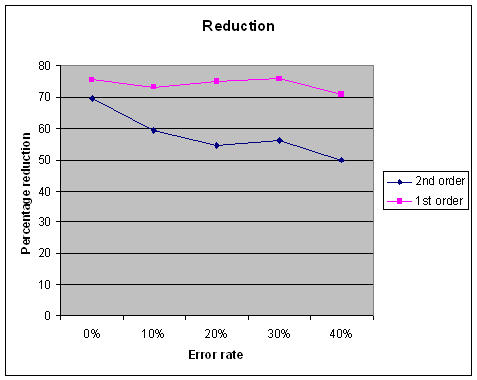
\includegraphics[scale=0.7]{xor_reduction} \end{center}

Uit de staafgrafieken blijkt dat voor de nauwkeurigheid in de xor-dataset gemiddeld het beste $k=1$ gebruikt kan worden voor het k-nearest-neighbour algoritme, als er weinig ruis in de dataset zit.  Als er veel ruis in de dataset zit, levert $k=5$ gemiddeld een zelfde of beter resultaat. Eerste orde editing levert gemiddeld een iets beter resultaat, vooral voor $k=1$. Eerste orde editing verwijdert meer punten, zeker bij meer ruis. 

\subsection{MNIST}

Van de MNIST-dataset was een trainset en een testset beschikbaar. We kregen de volgende resultaten:\\
\begin{tabular}{|c|c|c|c|c|}  \hline
	& Accuracy	&Accuracy &Accuracy &	Reduction \\ \hline
	& K=1 &	K=3 &	K=5	& \\ \hline
1ST order editing, 1ST order neighbour testing &	71,8	& 68,6	& 62	& 89,3 \\
1ST order editing, 2ND order neighbour testing &	71,8	& 69 &	64,4 &	89,3 \\
2ND order editing, 1ST order neighbour testing &	67,6	& 60,4 &	52,8 &	78,8 \\
2ND order editing, 2ND order neighbour testing &	67,6	& 60,4 &	54,6	& 78,8 \\ \hline
\end{tabular} \\
\begin{center} 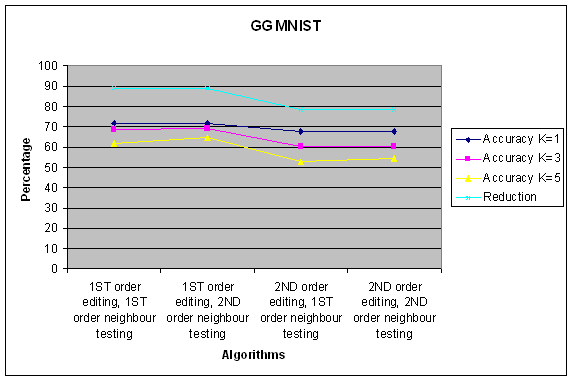
\includegraphics[scale=0.7]{GG_MNIST} \end{center}

Voor deze dataset blijven de nauwkeurigheid en reductie vrij stabiel, tweede orde editing is iets slechter. Voor alle gevallen geldt dat $k=1$ de beste keuze voor $k$ is.

\subsection{Diabetes}

Van de diabetes-dataset was een trainset en een testset beschikbaar. We kregen de volgende resultaten:\\
\begin{tabular}{|c|c|c|c|c|}  \hline
	& Accuracy	&Accuracy &Accuracy &	Reduction \\ \hline
	& K=1 &	K=3 &	K=5	& \\ \hline
1ST order editing, 1ST order neighbour testing &	78,9 &	78,1 &	77,3	& 49,2 \\
1ST order editing, 2ND order neighbour testing &	78,9 &	78,1 &	78,1 &	49,2 \\
2ND order editing, 1ST order neighbour testing &	73,4 &	78,9 &	79,7 &	37,5 \\
2ND order editing, 2ND order neighbour testing &	73,4 &	78,1 &	78,9 &	37,5 \\ \hline
\end{tabular} \\
\begin{center} 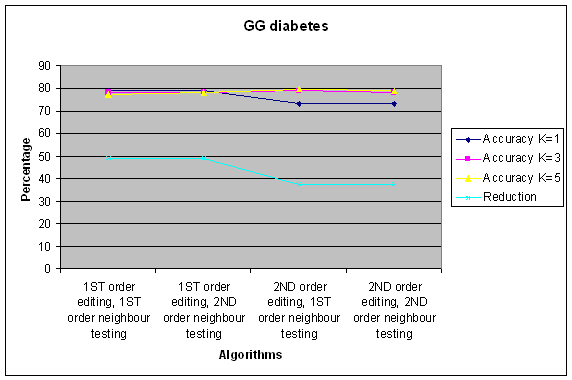
\includegraphics[scale=0.7]{GG_diabetes} \end{center}

Voor deze dataset liggen de resultaten voor $k=3$ en $k=5$ erg dicht bij elkaar, afhankelijk van het algoritme dat je kiest is de een of de ander beter. $k=1$ blijkt bij deze dataset juist een slechtere keuze te zijn.

%\subsection{RNG}
%\begin{tabular}{|c|c|c|c|c|c|c|c|c|c|}  \hline
%	 & &	Accuracy & Accuracy & Accuracy & 	reduction \\ \hline
%set &	orde &	K = 1 & 	K = 3 & 	K = 5	 &	\\ \hline
%xor &	1 &	65 &	60 &	60 &	21 \\
%diabetes &	1 &	71 &	74 &	73 &	18 \\
%mnist	 & 1 &	88 &	83 &	83 &	39 \\
%xor & 	2 &	85 &	70 &	70 &	35 \\
%diabetes &	2 &	65 &	68 &	68 &	49 \\
%mnist	 & 2 &	88 &	87 &	86 &	53 \\ \hline
%\end{tabular} \\

\subsection{Performance}
De performance van het algoritme hangt sterk af van het aantal punten in de trainset. Door de implementatie van het zoeken van edges in een graaf, is de complexiteit van het maken van een graaf $\theta (d\cdot N^3)$, waarbij d het aantal dimensies is en N het aantal punten in de trainset. Voor elke combinatie van twee punten wordt nu namelijk gekeken of ze buren zijn, door te zoeken naar een derde punt dat er tussenin ligt. Het maken van een proximity graph zou in $\theta (d\cdot N log N)$ moeten kunnen. Het maken van een prototype hoeft echter geen probleem te zijn: dit wordt eenmalig gedaan door een programma, waarna er onbeperkt geclassificeerd kan worden. De implementatie is nadeliger voor het testen van nieuwe punten. Dit heeft per nieuw punt complexiteit $\theta (d\cdot N^2)$, waarbij N de grootte van het prototype is. Hierdoor is de performance bij grote trainsets, zoals de MNIST-set, vrij slecht. De performance met trainsets en testsets met enkele honderden of minder punten is goed: dit gaat op een moderne computer in de orde van seconden. Om de performance van grotere sets wat te verbeteren is multithreading gebruikt, het algoritme leent zich goed voor een arbitrair aantal threads. Dit verlaagt de complexiteit echter niet en zou dus niet als significante verbetering van het algoritme gezien moeten worden. 

\section{Conclusie}
Proximity graphs zijn geschikt voor het toepassen van het kNN-principe. De effectiviteit verschilde per testset en per parameter in het algoritme. Bij de XOR-set en de diabetes-set was de het percentage fout gelabelde punten ongeveer gelijk aan het percentage ruis. Het editing-algoritme lukt het dus niet om de nauwkeurigheid in dat opzicht te verbeteren, maar het zorgt wel voor een reductie en daarmee voor een snellere uitvoering van het algoritme. Bij de MNIST-set was het percentage fouten 8\% tot 28\% hoger dan het percentage ruis, hierin was het editing-algoritme dus niet effectief. Een kleinere K gaf hierbij de beste resultaten. Eerste orde editing gaf in alle gevallen een gelijke of lagere nauwkeurigheid dan de tweede orde editing. De orde van testen heeft bij sommige datasets niet zo veel invloed, dit kan verklaard worden doordat het aantal buren van een punt vaak groter is dan k, waardoor tweede orde testing alleen tests doet met de directe buren, en dus vaak hetzelfde doet als eerste orde testing.

De reductie bij de simpele XOR-test lag tussen de 50\% en 76\%, waarbij met name de tweede orde editing niet veel reductie behaalde als er enige ruis aanwezig was. Dat eerste orde editing meer reductie behaalt komt doordat tweede orde editing test of het punt verwijderd zou worden met eerste orde editing, waarna het punt niet altijd verwijderd wordt als eerste orde editing dat zou doen, door de extra conditie van tweede orde editing. De reductie van de eerste-orde editing was voor alle hoeveelheden ruis vrij hoog, tussen de 70\% en 76\%. Ook bij de reductie van de MNIST-set en de diabetes-set was de eerste-orde editing ruim 10\% effectiever dan de tweede-orde editing. De reductie van MNIST lag vrij hoog, tussen de 78\% en 90\%, maar bij de diabetes-set kon weinig reductie bereikt worden, tussen de 37\% en 50\%. In sommige gevallen levert de reductie dus weinig ruimtebesparing op.

Omdat de nauwkeurigheid van eerste- en tweede-orde editing niet veel uiteen lopen, maar eerste-orde wel consistent meer reductie behaalt, lijkt dit dus onder verschillende omstandigheden het betere testcriterium te zijn.

De performance van het algoritme is voor grote testsets slecht, doordat de implementatie een complexiteit van $\theta (d\cdot N^3)$ heeft. Dit zou verbeterd kunnen worden door een ander algoritme te gebruiken om de buren van een punt te bepalen. Ook de methode voor de editing/condensing zou verbeterd kunnen worden, er is in sommige gevallen slechts weinig reductie waardoor de benodigde CPU-tijd voor het testen ook toeneemt. De nauwkeurigheid op testsets verschilt, voor MNIST is deze redelijk laag en voor grotere sets zou de nauwkeurigheid dus verbeterd mogen worden. Voor de XOR-set en de diabetes-set is de nauwkeurigheid goed.
\end{document}